\documentclass[12pt, a4paper, oneside]{ctexart}
\usepackage{amsmath, amsthm, amssymb, bm, graphicx, hyperref, mathrsfs}
\usepackage{tikz}
\usepackage{cite}
\usetikzlibrary{positioning} %为了实现相对位置的设定
\usepackage{xcolor} %为了实现不同的颜色
\title{\textbf{Homework 2: Navier Stokes}}
\date{\today}
\linespread{1}
\begin{document}

\maketitle
{\raggedright\subsection*{12.2 不可压缩Navier-Stokes方程}}
{\raggedright
不可压缩流体的二维流场完全由以下函数来描述, 速度矢量 {$ \ q=(u(x, y), v(x, y)) \in \mathbb{R}^2$} 
和压力{$\ p(x,y)\in \mathbb{R}$}。这些函数是以下守恒定律的解(例如,参照 Hirsch,1988):}\cite{book1}
\begin{itemize}
    \item[$\bullet$] 质量守恒定律:
    \begin{equation}
        \mathrm{div}(q)=0, \label{E1}
    \end{equation}
    或者使用散度\footnote{我们回顾一下二维场的微分算子散度、梯度和拉普拉斯算子的定义:如果$v=(v_x,v_y):\ \mathbb{R}^2\rightarrow \mathbb{R}^2$ 并且 $\varphi:
    \ \mathbb{R}^2\rightarrow \mathbb{R}$,那么$$
    \operatorname{div}(v)=\frac{\partial v_x}{\partial x}+\frac{\partial v_y}{\partial y}, \quad \mathcal{G} \varphi=\left(\frac{\partial \varphi}{\partial x}, \frac{\partial \varphi}{\partial y}\right), \quad \Delta \varphi=\operatorname{div}(\mathcal{G} \varphi)=\frac{\partial^2 \varphi}{\partial x^2}+\frac{\partial^2 \varphi}{\partial y^2},
    $$
    并且$\Delta v= (\Delta v_x,\Delta v_y)$。
    }运算符的显式形式,
    \begin{equation}
        \frac{\partial u}{\partial x}+\frac{\partial v}{\partial y}=0,\label{E2} 
    \end{equation}
    
    \item[$\bullet$] 简化形式的动量守恒定律 \footnote{我们用$\otimes$表示张量积。}
    \begin{equation}
        \frac{\partial q}{\partial t}+\mathrm{div}(q \otimes q)=-\mathcal{G} p+\frac{1}{R e} \Delta q \label{E3}
    \end{equation}
    或者使用显式形式,
    \begin{equation}
        \left\{\begin{array}{l}
            \frac{\partial u}{\partial t}+\frac{\partial u^2}{\partial x}+\frac{\partial u v}{\partial y}=-\frac{\partial p}{\partial x}+\frac{1}{R e}\left(\frac{\partial^2 u}{\partial x^2}+\frac{\partial^2 u}{\partial y^2}\right) \\
            \frac{\partial v}{\partial t}+\frac{\partial u v}{\partial x}+\frac{\partial v^2}{\partial y}=-\frac{\partial p}{\partial y}+\frac{1}{R e}\left(\frac{\partial^2 v}{\partial x^2}+\frac{\partial^2 v}{\partial y^2}\right)
            \end{array}\right.,\label{E4}
    \end{equation}
    \end{itemize}
    $ \ \ \ \ \ \    $ 以上方程使用以下缩放变量,按无因次形式编写:
    \begin{equation}
        x=\frac{x^*}{L},\  \ y=\frac{y^*}{L}, \ \ u=\frac{u^*}{L},\ \ v=\frac{v^*}{L},\ \ t=\frac{t^*}{L/V_0},\ \ p=\frac{p^*}{\rho_0 V_0^2},\label{E5}
    \end{equation}
    其中上标 \text{(*)}代表由物理单位度量的变量。常数$L,V_0$分别为表征模拟流动的参考长度和速度。无量纲数 Re 称为\emph{Reynolds 数},定量表示流动中的惯性(或对流)项和粘性(或扩散)\footnote{描述对流和扩散现象的模型标量方程已经在第 1 章中讨论过。}项的相对重要性:
    \begin{equation}
        Re =  \frac{V_0L}{\nu},\label{E6}
    \end{equation}
    其中$\nu$是流动的运动粘度。\\
    \text{  \  \ \  \ \ \ } 总之,本项目中,Navier–Stokes系统的偏微分方程形式,由 (2) 和 (4) 定义,将求出数值解;初始条件(t=0)和边界条件将在以下部分进行讨论。
{\raggedright\subsection*{12.4 计算域、交错网格和边界条件}}
{\raggedright
考虑处处具有周期性边界条件的矩形域$L_x×L_y$(见图1),Navier–Stokes方程的数值求解大大简化。
速度 $q(x, y)$ 和压力场 $p(x, y)$ 的周期性在数学上表示为:

}
\begin{equation}
    \begin{array}{lll}
        q(0, y)=q\left(L_x, y\right), & p(0, y)=p\left(L_x, y\right), & \forall y \in\left[0, L_y\right], \\
        q(x, 0)=q\left(x, L_y\right), & p(x, 0)=p\left(x, L_y\right), & \forall x \in\left[0, L_x\right].
        \end{array} \label{E7}
\end{equation}
\text{  \  \ \  \ \ \ }计算解决方案的点分布在均匀的矩形二维网格域内。由于在我们的方法中,并非所有变量都位于同一的网格,所以我们首先,定义一个一级网格(见图1)。
初始网格由沿$x$的$n_x$个计算点和沿$y$的$n_y$个计算点生成:

\begin{align}
& x_c(i)=(i-1) \delta x, \quad \delta x=\frac{L_x}{n_x-1}, \quad i=1, \ldots, n_x, \label{E8}\\
& y_c(j)=(j-1) \delta y, \quad \delta y=\frac{L_y}{n_y-1}, \quad j=1, \ldots, n_y .\label{E9}
\end{align}

\begin{figure}[h]
\centering

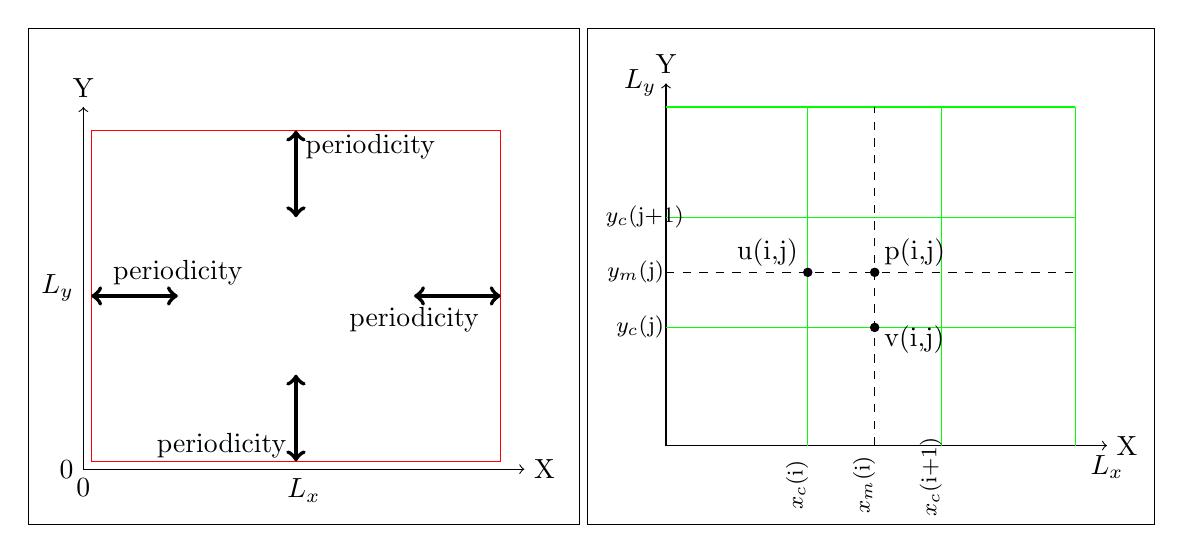
\begin{tikzpicture}
\draw(0,0)rectangle(7,6.3);% the first rectangle
\draw[->](0.7,0.7)--(6.3,0.7) node[right] {X};% x axis 
\draw[->](0.7,0.7)--(0.7,5.3) node[above] {Y};% y axis
\draw(3.5,0.7) node[below] {$L_x$};% x axis label
\draw(0.7,3) node[left] {$L_y$};% y axis label
\draw(0.7,0.7) node[below] {0};
\draw(0.7,0.7) node[left] {0};
\draw[red](0.8,0.8)rectangle(6,5);
\draw[line width=1.5pt][<->](0.8,2.9)--(1.9,2.9) node[above]{periodicity};
\draw[line width=1.5pt][<->](6,2.9)--(4.9,2.9) node[below]{periodicity};
\draw[line width=1.5pt][<->](3.4,5)--(3.4,3.9) ;
\draw[line width=1.5pt][<->](3.4,0.8)--(3.4,1.9) ;
\draw(3.4,1)node[left]{periodicity};
\draw(3.4,4.8)node[right]{periodicity};


\draw(7.1,0)rectangle(14.3,6.3);% the second rectangle
\draw[->](8.1,1)--(13.7,1) node[right] {X};% x axis 
\draw[->](8.1,1)--(8.1,5.6) node[above] {Y};% y axis
\draw(13.7,1) node[below] {$L_x$};% x axis label
\draw(8.1,5.6) node[left] {$L_y$};% y axis label
\draw[green](8.1,2.5)--(13.3,2.5);%green horizon line
\draw[green](8.1,3.9)--(13.3,3.9);
\draw[green](8.1,5.3)--(13.3,5.3);
\draw[green](9.9,1)--(9.9,5.3);%green vertical line
\draw[green](11.6,1)--(11.6,5.3);
\draw[green](13.3,1)--(13.3,5.3);
\draw[dashed](8.1,3.2)--(13.3,3.2);% dashed horizon line
\draw[dashed](10.75,1)--(10.75,5.3);% dashed vertical line
\draw[fill=black](9.9,3.2)circle[radius=1.5pt];
\draw(9.9,3.45) node[left]{u(i,j)};
\draw[fill=black](10.75,3.2)circle[radius=1.5pt];
\draw(10.75,3.45) node[right]{p(i,j)};
\draw[fill=black](10.75,2.5)circle[radius=1.5pt];
\draw(10.75,2.35) node[right]{v(i,j)};
\draw(8.2,2.5) node[left,font=\footnotesize]{$y_c$(j)};
\draw(8.2,3.2) node[left,font=\footnotesize]{$y_m$(j)};
\draw(8.45,3.9) node[left,font=\footnotesize]{$y_c$(j+1)};
\draw(9.5,0.5) node[below,rotate=90,font=\footnotesize]{$x_c$(i)};
\draw(10.35,0.5) node[below,rotate=90,font=\footnotesize]{$x_m$(i)};
\draw(11.2,0.6) node[below,rotate=90,font=\footnotesize]{$x_c$(i+1)};

\end{tikzpicture}
\caption{计算域、交错网格和边界条件} \label{fig:M1}
\end{figure}
\text{  \  \ \  \ \ \ }二级网格是由一级网格单元的中心定义的:
\begin{align}
    x_m(i)=(i-1 / 2) \delta x,\quad  & i=1, \ldots, n_{x m},\label{E10} \\
    y_m(j)=(j-1 / 2) \delta y,\quad  & j=1, \ldots, n_{y m},\label{E11}
\end{align}
其中我们使用了速记符号$n_{xm}=n_x-1,n_{ym}=n_y-1$。在由矩形$[x_c(i),x_c(i+1)]\times [y_c(i),y_c(i+1)]$定义的计算单元中,未知变量$u,v,p$ 将被计算为不同空间位置处解的近似值:
\\
\begin{itemize}
    \item[$\bullet$] $u(i,j)\approx u(x_c(i),y_m(j))$\ (单元的西面)
    \item[$\bullet$] $v(i,j)\approx v(x_m(i),y_c(j))$\ (单元的南面)
    \item[$\bullet$] $p(i,j)\approx p(x_m(i),y_m(j))$\ (单元的中心)
\end{itemize}
这种变量的交错排列具有压力和速度之间的强耦合的优点。它还有助于(参照本章末尾的参考资料)避免并置安排(所有变量在同一网格点处计算)中遇到的一些稳定性和收敛性问题。

\bibliographystyle{plain}
\bibliography{references}
\end{document}